% !TeX program = pdfLaTeX
\documentclass[12pt]{article}
\usepackage{amsmath}
\usepackage{graphicx,psfrag,epsf}
\usepackage{enumerate}
\usepackage{natbib}
\usepackage{textcomp}
\usepackage[hyphens]{url} % not crucial - just used below for the URL
\usepackage{hyperref}

%\pdfminorversion=4
% NOTE: To produce blinded version, replace "0" with "1" below.
\newcommand{\blind}{0}

% DON'T change margins - should be 1 inch all around.
\addtolength{\oddsidemargin}{-.5in}%
\addtolength{\evensidemargin}{-.5in}%
\addtolength{\textwidth}{1in}%
\addtolength{\textheight}{1.3in}%
\addtolength{\topmargin}{-.8in}%

%% load any required packages here


% Pandoc syntax highlighting
\usepackage{color}
\usepackage{fancyvrb}
\newcommand{\VerbBar}{|}
\newcommand{\VERB}{\Verb[commandchars=\\\{\}]}
\DefineVerbatimEnvironment{Highlighting}{Verbatim}{commandchars=\\\{\}}
% Add ',fontsize=\small' for more characters per line
\usepackage{framed}
\definecolor{shadecolor}{RGB}{248,248,248}
\newenvironment{Shaded}{\begin{snugshade}}{\end{snugshade}}
\newcommand{\AlertTok}[1]{\textcolor[rgb]{0.94,0.16,0.16}{#1}}
\newcommand{\AnnotationTok}[1]{\textcolor[rgb]{0.56,0.35,0.01}{\textbf{\textit{#1}}}}
\newcommand{\AttributeTok}[1]{\textcolor[rgb]{0.77,0.63,0.00}{#1}}
\newcommand{\BaseNTok}[1]{\textcolor[rgb]{0.00,0.00,0.81}{#1}}
\newcommand{\BuiltInTok}[1]{#1}
\newcommand{\CharTok}[1]{\textcolor[rgb]{0.31,0.60,0.02}{#1}}
\newcommand{\CommentTok}[1]{\textcolor[rgb]{0.56,0.35,0.01}{\textit{#1}}}
\newcommand{\CommentVarTok}[1]{\textcolor[rgb]{0.56,0.35,0.01}{\textbf{\textit{#1}}}}
\newcommand{\ConstantTok}[1]{\textcolor[rgb]{0.00,0.00,0.00}{#1}}
\newcommand{\ControlFlowTok}[1]{\textcolor[rgb]{0.13,0.29,0.53}{\textbf{#1}}}
\newcommand{\DataTypeTok}[1]{\textcolor[rgb]{0.13,0.29,0.53}{#1}}
\newcommand{\DecValTok}[1]{\textcolor[rgb]{0.00,0.00,0.81}{#1}}
\newcommand{\DocumentationTok}[1]{\textcolor[rgb]{0.56,0.35,0.01}{\textbf{\textit{#1}}}}
\newcommand{\ErrorTok}[1]{\textcolor[rgb]{0.64,0.00,0.00}{\textbf{#1}}}
\newcommand{\ExtensionTok}[1]{#1}
\newcommand{\FloatTok}[1]{\textcolor[rgb]{0.00,0.00,0.81}{#1}}
\newcommand{\FunctionTok}[1]{\textcolor[rgb]{0.00,0.00,0.00}{#1}}
\newcommand{\ImportTok}[1]{#1}
\newcommand{\InformationTok}[1]{\textcolor[rgb]{0.56,0.35,0.01}{\textbf{\textit{#1}}}}
\newcommand{\KeywordTok}[1]{\textcolor[rgb]{0.13,0.29,0.53}{\textbf{#1}}}
\newcommand{\NormalTok}[1]{#1}
\newcommand{\OperatorTok}[1]{\textcolor[rgb]{0.81,0.36,0.00}{\textbf{#1}}}
\newcommand{\OtherTok}[1]{\textcolor[rgb]{0.56,0.35,0.01}{#1}}
\newcommand{\PreprocessorTok}[1]{\textcolor[rgb]{0.56,0.35,0.01}{\textit{#1}}}
\newcommand{\RegionMarkerTok}[1]{#1}
\newcommand{\SpecialCharTok}[1]{\textcolor[rgb]{0.00,0.00,0.00}{#1}}
\newcommand{\SpecialStringTok}[1]{\textcolor[rgb]{0.31,0.60,0.02}{#1}}
\newcommand{\StringTok}[1]{\textcolor[rgb]{0.31,0.60,0.02}{#1}}
\newcommand{\VariableTok}[1]{\textcolor[rgb]{0.00,0.00,0.00}{#1}}
\newcommand{\VerbatimStringTok}[1]{\textcolor[rgb]{0.31,0.60,0.02}{#1}}
\newcommand{\WarningTok}[1]{\textcolor[rgb]{0.56,0.35,0.01}{\textbf{\textit{#1}}}}

% tightlist command for lists without linebreak
\providecommand{\tightlist}{%
  \setlength{\itemsep}{0pt}\setlength{\parskip}{0pt}}

% From pandoc table feature
\usepackage{longtable,booktabs,array}
\usepackage{calc} % for calculating minipage widths
% Correct order of tables after \paragraph or \subparagraph
\usepackage{etoolbox}
\makeatletter
\patchcmd\longtable{\par}{\if@noskipsec\mbox{}\fi\par}{}{}
\makeatother
% Allow footnotes in longtable head/foot
\IfFileExists{footnotehyper.sty}{\usepackage{footnotehyper}}{\usepackage{footnote}}
\makesavenoteenv{longtable}


\usepackage{booktabs}
\usepackage{longtable}
\usepackage{array}
\usepackage{multirow}
\usepackage{wrapfig}
\usepackage{float}
\usepackage{colortbl}
\usepackage{pdflscape}
\usepackage{tabu}
\usepackage{threeparttable}
\usepackage{threeparttablex}
\usepackage[normalem]{ulem}
\usepackage{makecell}
\usepackage{xcolor}

\begin{document}


\def\spacingset#1{\renewcommand{\baselinestretch}%
{#1}\small\normalsize} \spacingset{1}


%%%%%%%%%%%%%%%%%%%%%%%%%%%%%%%%%%%%%%%%%%%%%%%%%%%%%%%%%%%%%%%%%%%%%%%%%%%%%%

\if0\blind
{
  \title{\bf Three (Groups of) Blind Mice. Familial Clusters of Cataract Development in Irradiated Mice}

  \author{
        Alyssa Allsop and Amira Burns \\
    Department of Statistics, Colorado State University\\
      }
  \maketitle
} \fi

\if1\blind
{
  \bigskip
  \bigskip
  \bigskip
  \begin{center}
    {\LARGE\bf Three (Groups of) Blind Mice. Familial Clusters of Cataract Development in Irradiated Mice}
  \end{center}
  \medskip
} \fi

\bigskip
\begin{abstract}
As astronauts travel farther into space, outside of the earth's protective magnetic field, they are exposed to radiation that could have serious effects. One of those side effects is cataract development. It has also been thought that there might be a genetic predisposition to develop cataracts that is passed down in families. The goal of this study was to use mice in families exposed to radiation to determine if there is cataract clustering in families. A mixed effects model was created to account for the family effect on cataract development. The model included terms for sex, treatment group, sex by treatment group interaction, and a random intercept for family. Family was shown to be an important source of variation in predicting cataract development. Males had big differences in cataract development among treatment groups whereas females had only small differences. Males were also more likely to develop severe cataracts than females in all three treatment groups. Other risks involved in radiation exposure could cause death before cataracts have time to develop. This complicates the inferences made about cataract development from this dataset; however, the conclusions indicate the necessity of further research to better understand how humans might react to radiation as they leave the earth's magnetic field.
\end{abstract}

\noindent%
{\it Keywords:} Hierarchical modeling, Logistic Regression, Bayesian analysis
\vfill

\newpage
\spacingset{1.45} % DON'T change the spacing!

\section{Introduction}
\label{sec:intro}

Little is known about the effects of high atomic number and energy (HZE) radiation, a main component of space radiation to which exposure is unavoidable beyond Earth's magnetic field. In contrast, extensive research shows exposure to high doses of gamma radiation leads to acute radiation sickness. Effects include damage to the blood forming system, GI system, immune system, increased risk for cancer, cardiovascular disease, neurodegenerative disease, death, and cataracts. Adverse effects from radiation may also be attributable to other factors, including genetics; several different cancers have been observed to cluster in mice families \citep{mice2017}. Accounting for potential family clustering allows for thorough examination of the primary research questions.\\
Is there a genetic susceptibility to cataracts caused by radiation? Accounting for potential genetic susceptibility, is there a difference in cataract presentation between HZE radiation, gamma radiation and unirradiation? 1820 individual mice from 48 unique families, were randomly assigned with equal family weight to each of three treatment groups. The mice were bred over several generations to create a genetically heterogeneous sample to better represent biological diversity within the human population. The treatments are HZE irradiation, gamma irradiation, and non-irradiated control. The HZE group is irradiated with either silicon or iron nuclei HZE ions, which are considered as a single treatment group. The second group is subjected to 137 Cs gamma irradiation. Mice in both irradiated groups are exposed to radiation at 7-12 weeks of age. The third group is unirradiated control. All mice are monitored until 800 days of age --effectively a survival study. Mice are checked weekly for symptoms of cataracts, cataract risk factors, and other symptoms of radiation exposure such as tumors and carcinomas. Resources do not allow for weekly measurement of every mouse; previous measurements are carried forward if a mouse is not assessed on a particular week.\\
This analysis uses a simplified version of the data set - a snapshot of the 1169 mice that are alive at 552 days. This cutoff is chosen because it is the median survival time for the group with the shortest median survival. There are 47 unique families with n = 396 in the HZE group, n = 277 in the gamma radiation group, and n = 496 in the unirradiated control group. There are up to two generations of mice pups from each family in the dataset, but generation is not distinguished in the simplified data. Family size ranges from n = 11 to n = 48, with median family size of 24.

\begin{wraptable}{r}{0pt}
\centering
\begin{tabular}{lrrrrr}
  \toprule
\multicolumn{1}{c}{ } & \multicolumn{4}{c}{Cataract Score} & \multicolumn{1}{c}{ } \\
\cmidrule(l{3pt}r{3pt}){2-5}
Treatment & 1 & 2 & 3 & 4 & Total \\ 
  \midrule
Unirradiated & 438 &  45 &  11 &   2 & 496 \\ 
  Gamma & 214 &  53 &   6 &   4 & 277 \\ 
  HZE & 281 & 107 &   6 &   2 & 396 \\ 
   \bottomrule
\end{tabular}
\caption{Counts of score by treatment group} 
\end{wraptable}

The response is a discrete ordinal variable corresponding to radiation-associated ocular changes in the eye. A score of 0 is associated with a completely clear lens, while a score of 5 is associated with a completely occluded lens. This dataset contains cataract score levels = {[}1, 2, 3, 4{]}. A score \(\ge\) 2 indicates presence of cataracts, and the small sample sizes for score \(>\) 2 across all treatment groups raise concerns about making inference on an ordinal analysis; consequently, the response is converted to binary \emph{Cataracts} with score = 1 converted to 0, and score \(\ge\) 2 converted to 1. The main experimental factor is \emph{Treatment}, a categorical variable with three levels = {[}HZE radiation, gamma radiation, non-irradiated control{]}. A single random effect, genetic \emph{Family}, is a categorical factor with 47 levels. Both Treatment and Family are central to the experimental design and will serve as the basis for all models considered. Additional covariates under consideration were Sex, coat color, weight in grams, body condition score (BCS) age in days, and presence three cancers: myeloid leukemia, harderian tumors, and PreT lymphoma. The experimental design prescribed the inclusion of Treatment and Family in the analysis.

\section{Summary Statistics}
\label{sec:sumstats}

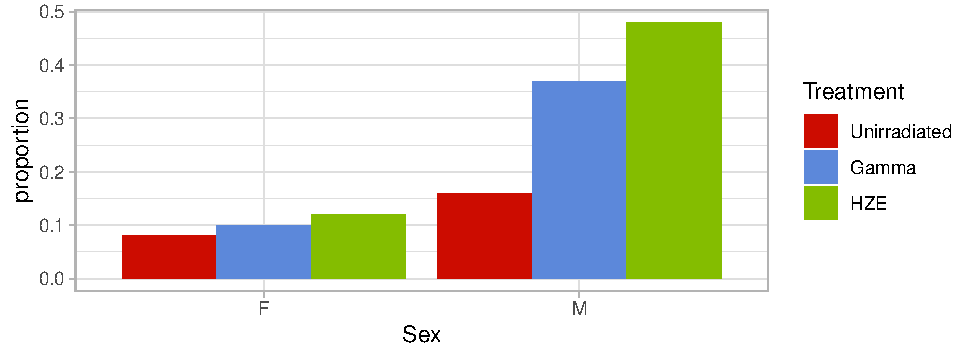
\includegraphics{bookdown_report_files/figure-latex/bareda-1.pdf}
Exploratory data analysis focused on assessing binary Cataracts status in terms of Treatment. Tables and graphs were produced to investigate any potential associations between covariates and the response, and correlations between coviarates and either Treatment or the response. Further examination of potential covariates show distinct patterns of cataracts status between male and female mice. Figure \ref{fig:bareda} highlights the differences between males and females across all treatment groups.

Figure \ref{fig:lineeda} allows us to visualize any patterns between families within other predictors of interest. Different patterns are displayed across families, but distinct clustering is not apparent.\\
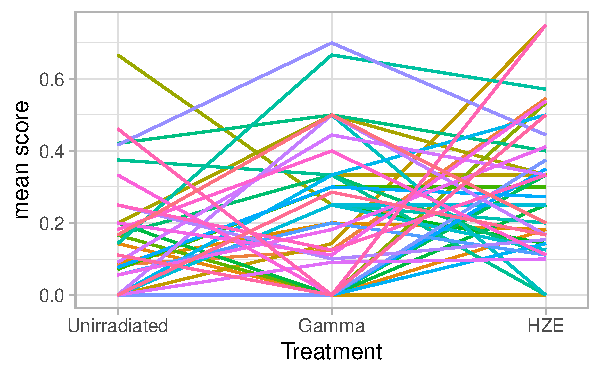
\includegraphics{bookdown_report_files/figure-latex/lineeda-1.pdf}

\section{Statistical Methods}
\label{sec:methods}

Hierarchical logistic regression was selected as the primary analysis method, due to the binary response and random effect of interest to the research question. Figure \ref{fig:bareda} indicated potential interaction between Sex and Treatment group; therefore, an interaction term was included in the model. Various models were fit and assessed using Aikike's Information Criterion (AIC); the full list of models fit can be viewed in Appendix Table \ref{glmms}.The final model, Model \eqref{eq:glmm}, can be written as:

\begin{equation}
\begin{aligned}
Y_{ij} \sim &Bernoulli(p) \\
log(\frac{p}{1-p}) = &\ \beta_0\ +\beta_1*Gamma_i\ + \beta_2*HZE_i\ + \beta_3*M_i\ + \\ &\beta_4*Gamma_i*M_i\ + \beta_5*HZE_i*M_i\ +\ [v_{j} + \epsilon_{ij}] \\
&i = 1, ..., 1169\ \mbox{ mice} \\
&j = 1,...,47\ \ \mbox{ families}
\end{aligned}
\label{eq:glmm}
\end{equation}

where \(M_i\) is an indicator for males, \(v_{j}\) is the variance of the random intercept for Family \(j\), and \(\epsilon_{ij}\) is the residual variance.

A complementary Bayesian model with non-informative priors was fit to examine the distribution of the estimates from the final model, as well as test its robustness to alternative approaches \citep{BDA}. The Bayes model is parameterized as:\\
\begin{equation}
\begin{aligned}
Y_{ij} \sim &Bernoulli(p)\\
log(\frac{p}{1-p}) = &\ \beta_0*Control_i*F_i\ +\beta_1*Gamma_i*F_i\ + \beta_2*HZE_i*F_i\ + \\ &\beta_3*Control_i*M_i\ +\beta_4*Gamma*M\ + \beta_5*HZE*M\ + \\
&v_{j} + \epsilon_{ij}\\
&i = 1, ..., 1169\ \mbox{ mice} \\
&j = 1,...,47\ \ \mbox{ families, and} \\
v_j \sim\ &N(0, \tau)
\\
&\mbox{ with non-informative priors:}\\
\beta_0 &\sim N(0, 0.001)\ \ \ \ \beta_1 \sim N(0, 0.001)\ \ \ \ \beta_2 \sim N(0, 0.001)\\
\beta_3 &\sim N(0, 0.001)\ \ \ \ \beta_4 \sim N(0, 0.001)\ \ \ \ \beta_5 \sim N(0, 0.001)\\
v_i &\sim N(0, \sigma^2)\\
\tau &\sim Gamma(0.001, 0.001) \mbox{ where}\ \sigma^2 = 1/\tau 
\end{aligned}
\label{eq:bayes}
\end{equation}

Model \eqref{eq:bayes}, was run through a Gibbs sampler Markov Chain Monte Carlo (MCMC) algorithm in the \texttt{rjags} package \citep{R-rjags} to approximate the posterior distributions of the estimates of all fixed effects and the variance of the random effect. 3 chains of 60000 total iterations with a 10000-iteration burn-in period; starting values were obtained from the estimates generated by Model \eqref{eq:glmm}, with random noise added to avoid false convergence.

Estimates for the final analysis:

\begin{table}[H]
\centering
\begin{tabular}{rrrrr}
  \toprule
GLMM Est & MCMC Mode & MCMC SD & HPD Lower & HPD Upper \\ 
  \midrule
-2.70 & -2.68 & 0.27 & -3.25 & -2.20 \\ 
  0.21 & 0.09 & 0.38 & -0.53 & 0.95 \\ 
  0.50 & 0.49 & 0.33 & -0.14 & 1.15 \\ 
  0.89 & 0.90 & 0.30 & 0.31 & 1.50 \\ 
  0.97 & 1.09 & 0.46 & 0.08 & 1.88 \\ 
  1.21 & 1.27 & 0.41 & 0.40 & 2.00 \\ 
  0.40 & 0.32 & 0.18 & 0.15 & 0.81 \\ 
   \bottomrule
\end{tabular}
\caption{Final model parameter estimates} 
\end{table}

The 95\% highest posterior density (HPD) credible intervals from Model \eqref{eq:bayes}

\section{Limitations and Alternatives}
\label{sec:limits}

Logistic regression assumes linearity of \(log(\frac{p}{1-p})\) \citep{BMLR2021}.
Limitations include lack of robust diagnostic assessment of GLMMs \citep{CDA}.
Presence of competing risks in the experimental design obscure the presence of family clusters of cataracts. Simplifying the dataset by instituting a cutoff age attempts to address this limitation, but the issue persists even after excluding individuals deceased before Age = 552.

\section{Results}
\label{sec:results}

The final probability for developing cataracts can be written as:\\
\begin{equation}
\begin{aligned}
p_i = &0.063 + 0.55*Gamma_i + 0.623*HZE_i + \\
&0.708*Male_i + 0.726*Gamma_i*Male_i + 0.770*HZE_i*Male_i
\end{aligned}
\label{eq:probs}
\end{equation}

Comparisons of different groups across Sex and Treatment were assessed on Model \eqref{eq:glmm} using the \texttt{emmeans} package \citep{R-emmeans}. Figure \ref{fig:contr} shows the probability of developing cataracts for each combination of sex by treatment group. Differences between both sex and treatment group are clearly visible, notably the differences between treatment group across gender.

\begin{figure}[H]

{\centering 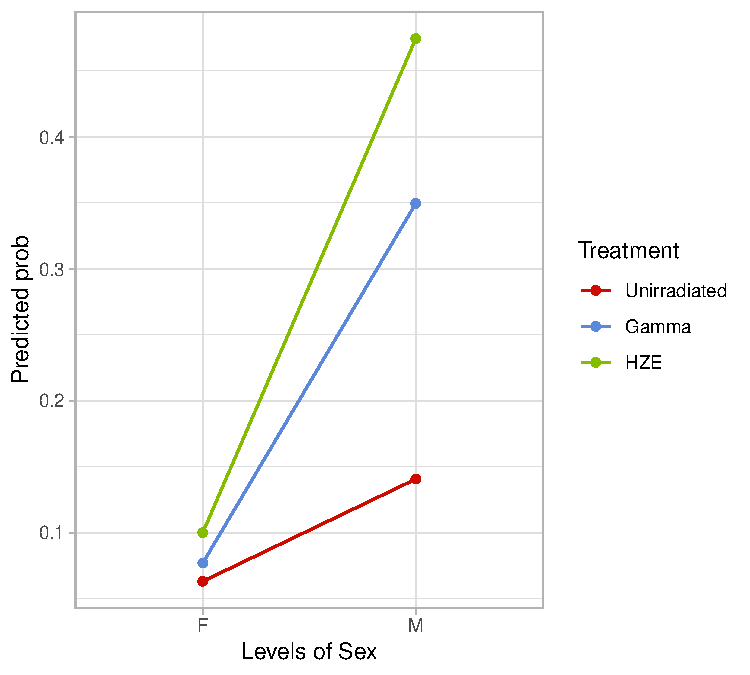
\includegraphics{bookdown_report_files/figure-latex/contr-1} 

}

\caption{Predicted probability of cataracts by sex, treatment group}\label{fig:contr}
\end{figure}

Assessing relative risk for cataracts between groups:\\

\begin{figure}[H]
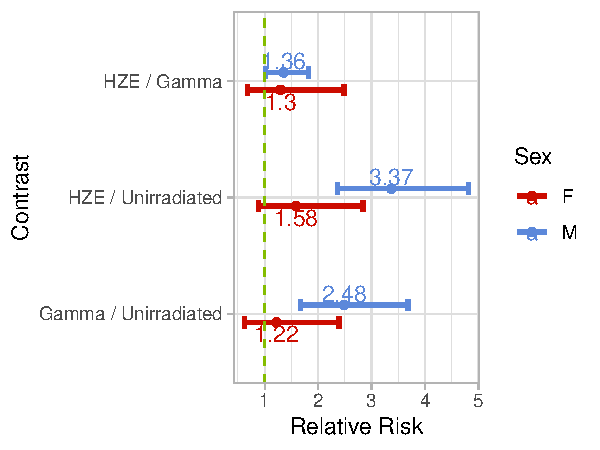
\includegraphics[width=0.5\linewidth]{bookdown_report_files/figure-latex/RR-1} 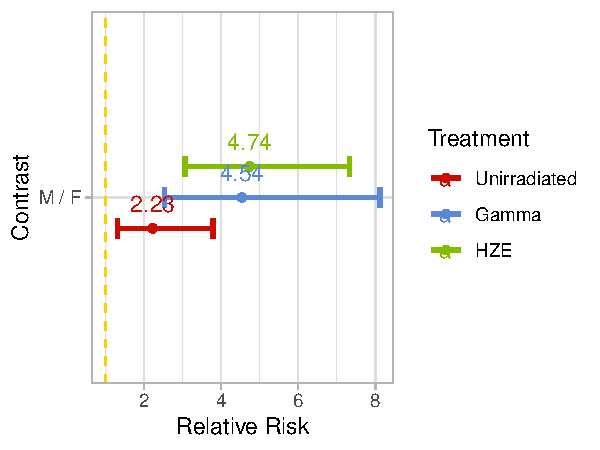
\includegraphics[width=0.5\linewidth]{bookdown_report_files/figure-latex/RR-2} \caption{Relative risk of cataract development by all predictor combinations}\label{fig:RR}
\end{figure}

Fix this plot!

\begin{figure}[H]

{\centering 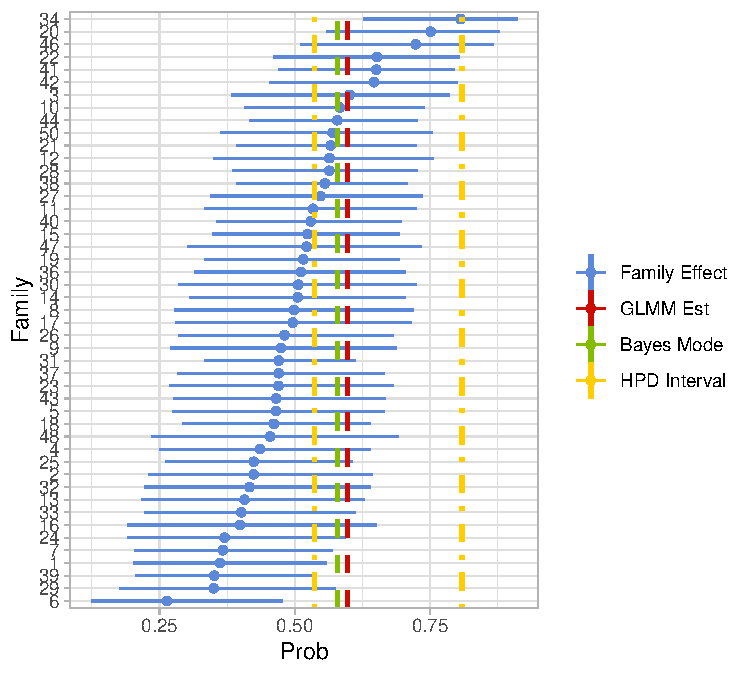
\includegraphics{bookdown_report_files/figure-latex/re-1} 

}

\caption{Estimated random probability of developing cataracts by family}\label{fig:re}
\end{figure}

Figure \ref{fig:re} visualizes the estimated probability of developing cataracts for each family in the dataset, along with their confidence intervals. The vertical lines plot the GLMM estimated variance from Model \eqref{eq:glmm} and the MCMC mode and HPD interval for \(\sigma^2\) from Model \eqref{eq:bayes}. Many of the probabilities shown are close to 0.5, with small numbers of families at the top and bottom of the graph that indicate some respective genetic predisposition or resistance to cataract development.

\section{Conclusions}
\label{sec:conc}

\textbf{Turn this into a nice paragraph or two; add quantitative info from results to back these up, or keep it general?}

Females in general face less probability of developing cataracts than males, across all treatment groups. We could argue that the effect of treatment group is not of clinical significance for female mice in this dataset. As you can see, the probability of developing cataracts is quite low for all 3 treatment groups. Males, on the other hand, have a higher probability of developing cataracts than females across all treatment groups. For males, the differences of development of cataracts across treatment groups is of clinical importance.

\section{Author's Statements}
\label{sec:auth}

Both authors contributed to statistical analysis and writing for this report. Both authors read and approved the final report. Both authors contributed equally to introduction, exploratory data analysis, summary statistics, and results. Alyssa Allsop served as the primary statistician on fitting Frequentist models; Amira Burns served as the primary statistician on fitting the Bayesian model.

\section{Appendix}
\label{sec:appendix}

\hypertarget{additional-exploratory-data-analysis}{%
\subsubsection{Additional Exploratory Data Analysis}\label{additional-exploratory-data-analysis}}

\hypertarget{model-selection}{%
\subsubsection{Model Selection}\label{model-selection}}

AIC was used as the primary model selection criteria because it accurately compares non-nested models. This feature was of particular importance when assessing models with a random effect against a model with only fixed effects.

\begin{table}[!h]
\centering
\begin{tabular}{ll}
  \toprule
Model & AIC \\ 
  \midrule
Full Mixed Model & 1017.98 \\ 
  Final Model & 1038.9 \\ 
  Fixed Effects Model & 1040.3 \\ 
  Mixed Model with no Interaction & 1023.19 \\ 
  Base Model & 1123.57 \\ 
   \bottomrule
\end{tabular}
\caption{Model selection via AIC comparision} 
\end{table}

\hypertarget{bayesian-model-diagnostics}{%
\subsubsection{Bayesian Model Diagnostics}\label{bayesian-model-diagnostics}}

\hypertarget{source-code}{%
\subsubsection{Source Code}\label{source-code}}

\begin{Shaded}
\begin{Highlighting}[]
\NormalTok{knitr}\SpecialCharTok{::}\NormalTok{opts\_chunk}\SpecialCharTok{$}\FunctionTok{set}\NormalTok{(}\AttributeTok{fig.width=}\DecValTok{4}\NormalTok{, }\AttributeTok{fig.height =} \DecValTok{4}\NormalTok{, }\AttributeTok{fig.pos =} \StringTok{\textquotesingle{}H\textquotesingle{}}\NormalTok{,}
                      \AttributeTok{echo=}\ConstantTok{FALSE}\NormalTok{, }\AttributeTok{warning=}\ConstantTok{FALSE}\NormalTok{, }\AttributeTok{message=}\ConstantTok{FALSE}\NormalTok{) }

\FunctionTok{library}\NormalTok{(readxl)}
\FunctionTok{library}\NormalTok{(tidyverse)}
\FunctionTok{library}\NormalTok{(lme4)}
\FunctionTok{library}\NormalTok{(broom.mixed)}
\FunctionTok{library}\NormalTok{(kableExtra)}
\FunctionTok{library}\NormalTok{(xtable)}
\FunctionTok{library}\NormalTok{(emmeans)}
\FunctionTok{library}\NormalTok{(ggsci)}
\FunctionTok{library}\NormalTok{(sjPlot)}
\FunctionTok{library}\NormalTok{(coda)}
\FunctionTok{library}\NormalTok{(rjags)}
\FunctionTok{library}\NormalTok{(R2jags)}
\FunctionTok{library}\NormalTok{(superdiag)}
\FunctionTok{library}\NormalTok{(mcmcplots)}
\FunctionTok{library}\NormalTok{(ggmcmc)}
\FunctionTok{library}\NormalTok{(gridExtra)}
\NormalTok{cats }\OtherTok{\textless{}{-}} \FunctionTok{read\_excel}\NormalTok{(}\AttributeTok{path =} \StringTok{"GRSD.cataract.xlsx"}\NormalTok{, }\AttributeTok{sheet =} \StringTok{"Sheet1"}\NormalTok{)}
\CommentTok{\# remove spaces from column and value names}
\FunctionTok{names}\NormalTok{(cats) }\OtherTok{\textless{}{-}} \FunctionTok{str\_replace\_all}\NormalTok{(}\FunctionTok{names}\NormalTok{(cats), }\StringTok{" "}\NormalTok{, }\StringTok{"\_"}\NormalTok{)}
\NormalTok{cats }\OtherTok{\textless{}{-}}\NormalTok{ cats }\SpecialCharTok{\%\textgreater{}\%}
  \FunctionTok{mutate}\NormalTok{(}\AttributeTok{CoatColor =} \FunctionTok{str\_replace\_all}\NormalTok{(coat\_color, }\StringTok{" "}\NormalTok{, }\StringTok{"\_"}\NormalTok{))}

\CommentTok{\# turn categorical vars into factor}
\NormalTok{cats }\OtherTok{\textless{}{-}}\NormalTok{ cats }\SpecialCharTok{\%\textgreater{}\%}
  \FunctionTok{rename}\NormalTok{(}\AttributeTok{Age =} \StringTok{\textasciigrave{}}\AttributeTok{age\_(days)}\StringTok{\textasciigrave{}}\NormalTok{,}
         \AttributeTok{Weight =}\NormalTok{ weight,}
         \AttributeTok{Animal =}\NormalTok{ animal) }\SpecialCharTok{\%\textgreater{}\%}
  \FunctionTok{mutate}\NormalTok{(}\AttributeTok{Sex =} \FunctionTok{as.factor}\NormalTok{(sex),}
         \AttributeTok{CoatColor =} \FunctionTok{as.factor}\NormalTok{(CoatColor),}
         \AttributeTok{Family =} \FunctionTok{as.factor}\NormalTok{(family), }\CommentTok{\# should this stay a factor? Yes?}
         \AttributeTok{BCS =} \FunctionTok{as.ordered}\NormalTok{(BCS),}
         \AttributeTok{Treatment =} \FunctionTok{relevel}\NormalTok{(}\FunctionTok{as.factor}\NormalTok{(groups), }\AttributeTok{ref =} \StringTok{"Unirradiated"}\NormalTok{),}
         \AttributeTok{MyeloidLeukemia =} \FunctionTok{as.factor}\NormalTok{(Myeloid\_Leukemia),}
         \AttributeTok{HarderianTumor =} \FunctionTok{as.factor}\NormalTok{(Harderian\_Tumor),}
         \AttributeTok{PreTLymphoma =} \FunctionTok{as.factor}\NormalTok{(PreT\_Lymphoma),}
         \AttributeTok{Score =} \FunctionTok{as.ordered}\NormalTok{(Cataract\_Score)) }\CommentTok{\# ordinal cat; leave as numeric?}

\CommentTok{\# select vars, add binary conversion for score}
\NormalTok{cats }\OtherTok{\textless{}{-}}\NormalTok{ cats }\SpecialCharTok{\%\textgreater{}\%}
  \FunctionTok{select}\NormalTok{(}\FunctionTok{c}\NormalTok{(Animal, Sex, Weight, CoatColor, Family, BCS, Age, Treatment,}
\NormalTok{           MyeloidLeukemia, HarderianTumor, PreTLymphoma, Score)) }\SpecialCharTok{\%\textgreater{}\%}
  \FunctionTok{mutate}\NormalTok{(}\AttributeTok{Cataracts =} \FunctionTok{ifelse}\NormalTok{(Score }\SpecialCharTok{\textless{}} \DecValTok{2}\NormalTok{, }\DecValTok{0}\NormalTok{, }\DecValTok{1}\NormalTok{))}

\CommentTok{\# glance at the dataset}
\CommentTok{\# str(cats)}
\NormalTok{gsc }\OtherTok{\textless{}{-}}\NormalTok{ cats }\SpecialCharTok{\%\textgreater{}\%} \FunctionTok{group\_by}\NormalTok{(Score) }\SpecialCharTok{\%\textgreater{}\%}
  \FunctionTok{count}\NormalTok{(Treatment) }\SpecialCharTok{\%\textgreater{}\%}
  \FunctionTok{pivot\_wider}\NormalTok{(}\AttributeTok{names\_from =}\NormalTok{ Score, }\AttributeTok{values\_from =}\NormalTok{ n) }\SpecialCharTok{\%\textgreater{}\%}
  \FunctionTok{group\_by}\NormalTok{(Treatment) }\SpecialCharTok{\%\textgreater{}\%}
  \FunctionTok{mutate}\NormalTok{(}\AttributeTok{Total =} \FunctionTok{sum}\NormalTok{(}\FunctionTok{c}\NormalTok{(}\StringTok{\textasciigrave{}}\AttributeTok{1}\StringTok{\textasciigrave{}}\NormalTok{, }\StringTok{\textasciigrave{}}\AttributeTok{2}\StringTok{\textasciigrave{}}\NormalTok{, }\StringTok{\textasciigrave{}}\AttributeTok{3}\StringTok{\textasciigrave{}}\NormalTok{, }\StringTok{\textasciigrave{}}\AttributeTok{4}\StringTok{\textasciigrave{}}\NormalTok{)))}

\FunctionTok{xtable}\NormalTok{(gsc, }\AttributeTok{caption =} \StringTok{"Counts of score by treatment group"}\NormalTok{) }\SpecialCharTok{\%\textgreater{}\%}
  \FunctionTok{xtable2kable}\NormalTok{(}\AttributeTok{booktabs =}\NormalTok{ T,}
               \AttributeTok{include.rownames =} \ConstantTok{FALSE}\NormalTok{,}
               \AttributeTok{table.placement =} \ConstantTok{NULL}\NormalTok{) }\SpecialCharTok{\%\textgreater{}\%}
  \FunctionTok{add\_header\_above}\NormalTok{(}\FunctionTok{c}\NormalTok{( }\StringTok{" "} \OtherTok{=} \DecValTok{1}\NormalTok{, }\StringTok{"Cataract Score"} \OtherTok{=} \DecValTok{4}\NormalTok{, }\StringTok{" "} \OtherTok{=} \DecValTok{1}\NormalTok{)) }\SpecialCharTok{\%\textgreater{}\%}
  \FunctionTok{kable\_styling}\NormalTok{(}\AttributeTok{full\_width =}\NormalTok{ F, }\AttributeTok{position =} \StringTok{"float\_right"}\NormalTok{) }
\CommentTok{\# barplot of proportion of each group with cataracts}
\NormalTok{sex\_trt }\OtherTok{\textless{}{-}}\NormalTok{ cats }\SpecialCharTok{\%\textgreater{}\%}
  \FunctionTok{group\_by}\NormalTok{(Treatment, Sex, Cataracts) }\SpecialCharTok{\%\textgreater{}\%}
  \FunctionTok{summarise}\NormalTok{(}\AttributeTok{n =} \FunctionTok{n}\NormalTok{()) }\SpecialCharTok{\%\textgreater{}\%}
  \FunctionTok{ungroup}\NormalTok{() }\SpecialCharTok{\%\textgreater{}\%}
  \FunctionTok{group\_by}\NormalTok{(Treatment, Sex) }\SpecialCharTok{\%\textgreater{}\%}
  \FunctionTok{mutate}\NormalTok{(}\AttributeTok{proportion =} \FunctionTok{round}\NormalTok{(n}\SpecialCharTok{/}\FunctionTok{sum}\NormalTok{(n), }\AttributeTok{digits =} \DecValTok{2}\NormalTok{))}

\NormalTok{cats\_grp }\OtherTok{\textless{}{-}}\NormalTok{ sex\_trt }\SpecialCharTok{\%\textgreater{}\%}
  \FunctionTok{filter}\NormalTok{(Cataracts }\SpecialCharTok{==} \DecValTok{1}\NormalTok{)}

\NormalTok{b1 }\OtherTok{\textless{}{-}} \FunctionTok{ggplot}\NormalTok{(cats\_grp, }\FunctionTok{aes}\NormalTok{(}\AttributeTok{x =}\NormalTok{ Sex, }\AttributeTok{y =}\NormalTok{ proportion, }\AttributeTok{fill =}\NormalTok{ Treatment)) }\SpecialCharTok{+}
  \FunctionTok{geom\_col}\NormalTok{(}\AttributeTok{position =} \StringTok{"dodge"}\NormalTok{) }\SpecialCharTok{+}
  \FunctionTok{scale\_fill\_startrek}\NormalTok{() }\SpecialCharTok{+}
  \FunctionTok{theme\_light}\NormalTok{() }

\NormalTok{b1}
\CommentTok{\# Plot of average score of sex{-}group{-}family}
\NormalTok{grsex\_score }\OtherTok{\textless{}{-}}\NormalTok{ cats }\SpecialCharTok{\%\textgreater{}\%}
  \FunctionTok{group\_by}\NormalTok{(Sex, Treatment, Family) }\SpecialCharTok{\%\textgreater{}\%}
  \FunctionTok{summarize}\NormalTok{(}\AttributeTok{mean\_score =} \FunctionTok{mean}\NormalTok{(Cataracts))}

\CommentTok{\# choose facet direction and just show one}
\NormalTok{l1 }\OtherTok{\textless{}{-}} \FunctionTok{ggplot}\NormalTok{(grsex\_score, }\FunctionTok{aes}\NormalTok{(}\AttributeTok{x =}\NormalTok{ Treatment, }\AttributeTok{y =}\NormalTok{ mean\_score, }\AttributeTok{color =}\NormalTok{ Sex)) }\SpecialCharTok{+}
  \FunctionTok{geom\_line}\NormalTok{(}\FunctionTok{aes}\NormalTok{(}\AttributeTok{group =}\NormalTok{ Family)) }\SpecialCharTok{+} \FunctionTok{facet\_grid}\NormalTok{(}\FunctionTok{vars}\NormalTok{(Sex)) }\SpecialCharTok{+}
  \FunctionTok{scale\_color\_startrek}\NormalTok{() }\SpecialCharTok{+}
  \FunctionTok{scale\_x\_discrete}\NormalTok{(}\AttributeTok{expand =} \FunctionTok{c}\NormalTok{(}\DecValTok{0}\NormalTok{, .}\DecValTok{2}\NormalTok{)) }\SpecialCharTok{+}
  \FunctionTok{theme\_light}\NormalTok{() }\SpecialCharTok{+}
  \FunctionTok{labs}\NormalTok{(}\AttributeTok{y =} \StringTok{"mean score"}\NormalTok{,}
       \AttributeTok{title =} \StringTok{"Cataracts by Family, Sex, Treatment Group"}\NormalTok{)}

\NormalTok{l1}
\NormalTok{mod }\OtherTok{\textless{}{-}} \FunctionTok{glmer}\NormalTok{(Cataracts }\SpecialCharTok{\textasciitilde{}}\NormalTok{ Treatment}\SpecialCharTok{*}\NormalTok{Sex }\SpecialCharTok{+}\NormalTok{ (}\DecValTok{1}\SpecialCharTok{|}\NormalTok{Family), }\AttributeTok{data =}\NormalTok{ cats, }\AttributeTok{family =}\NormalTok{ binomial)}
\CommentTok{\# Specify the model}
\FunctionTok{cat}\NormalTok{(}\StringTok{"model\{}
\StringTok{  for(i in 1:N)\{}
\StringTok{    CAT[i] \textasciitilde{} dbern(p[i])     \# Bernoulli{-}distributed response}
\StringTok{    logit(p[i])\textless{}{-} b0+ b1*Gamma[i] + b2*HZE[i] + b3*Male[i] +}
\StringTok{    b4*Male[i]*Gamma[i] + b5*Male[i]*HZE[i] + a[Family[i]]   \# likelihood function}
\StringTok{  \}}
\StringTok{  for(j in 1:nFam)\{}
\StringTok{    a[j] \textasciitilde{} dnorm(0, tau)}
\StringTok{  \}}
\StringTok{  b0 \textasciitilde{} dnorm(0.0, 1.0E{-}3)   \# vaguely informative priors}
\StringTok{  b1 \textasciitilde{} dnorm(0.0, 1.0E{-}3)}
\StringTok{  b2 \textasciitilde{} dnorm(0.0, 1.0E{-}3)}
\StringTok{  b3 \textasciitilde{} dnorm(0.0, 1.0E{-}3)}
\StringTok{  b4 \textasciitilde{} dnorm(0.0, 1.0E{-}3)}
\StringTok{  b5 \textasciitilde{} dnorm(0.0, 1.0E{-}3)}
\StringTok{  tau \textasciitilde{} dgamma(1.0E{-}3,1.0E{-}3)}
\StringTok{  sigma2 \textless{}{-} 1/tau     \# convert precision \textquotesingle{}tau\textquotesingle{} to variance \textquotesingle{}sigma2\textquotesingle{}}
\StringTok{\}"}\NormalTok{, }\AttributeTok{file =} \StringTok{"cat.jag"}\NormalTok{)}

\CommentTok{\# Prepare the data for JAGS}
\CommentTok{\# break Treatment into dummy variables for each group}
\NormalTok{treatment }\OtherTok{\textless{}{-}} \FunctionTok{model.matrix}\NormalTok{(}\SpecialCharTok{\textasciitilde{}}\NormalTok{ Treatment }\SpecialCharTok{{-}} \DecValTok{1}\NormalTok{, cats)}
\NormalTok{sex }\OtherTok{\textless{}{-}} \FunctionTok{model.matrix}\NormalTok{(}\SpecialCharTok{\textasciitilde{}}\NormalTok{Sex }\SpecialCharTok{{-}}\DecValTok{1}\NormalTok{, cats)}
\FunctionTok{colnames}\NormalTok{(treatment) }\OtherTok{\textless{}{-}} \FunctionTok{c}\NormalTok{(}\StringTok{"Unirradiated"}\NormalTok{, }\StringTok{"Gamma"}\NormalTok{, }\StringTok{"HZE"}\NormalTok{)}
\NormalTok{cats }\OtherTok{\textless{}{-}} \FunctionTok{data.frame}\NormalTok{(cats, treatment, sex)}

\CommentTok{\# format relevant data as a list}
\NormalTok{data }\OtherTok{\textless{}{-}} \FunctionTok{list}\NormalTok{(}\AttributeTok{CAT =}\NormalTok{ cats}\SpecialCharTok{$}\NormalTok{Cataracts, }\AttributeTok{Gamma =}\NormalTok{ cats}\SpecialCharTok{$}\NormalTok{Gamma, }
             \AttributeTok{HZE =}\NormalTok{ cats}\SpecialCharTok{$}\NormalTok{HZE, }\AttributeTok{Male =}\NormalTok{ cats}\SpecialCharTok{$}\NormalTok{SexM, }\AttributeTok{Family =}\NormalTok{ cats}\SpecialCharTok{$}\NormalTok{Family, }
             \AttributeTok{nFam =} \FunctionTok{length}\NormalTok{(}\FunctionTok{unique}\NormalTok{(cats}\SpecialCharTok{$}\NormalTok{Family)), }\AttributeTok{N =} \FunctionTok{nrow}\NormalTok{(cats))}

\NormalTok{nIter }\OtherTok{\textless{}{-}} \DecValTok{60000}
\NormalTok{nChains }\OtherTok{\textless{}{-}} \DecValTok{3}
\NormalTok{nThin }\OtherTok{\textless{}{-}} \DecValTok{1}
\NormalTok{BurnIn }\OtherTok{\textless{}{-}} \DecValTok{10000}
\NormalTok{nAdapt }\OtherTok{\textless{}{-}} \DecValTok{1000}
\NormalTok{ests }\OtherTok{\textless{}{-}} \FunctionTok{summary}\NormalTok{(mod)}\SpecialCharTok{$}\NormalTok{coef[,}\DecValTok{1}\NormalTok{] }\CommentTok{\# pull starting values from frequentist model}
\NormalTok{var }\OtherTok{\textless{}{-}} \FunctionTok{as.numeric}\NormalTok{(}\FunctionTok{as.data.frame}\NormalTok{(}\FunctionTok{VarCorr}\NormalTok{(mod))}\SpecialCharTok{$}\NormalTok{vcov)}
\NormalTok{inits }\OtherTok{\textless{}{-}} \FunctionTok{list}\NormalTok{(}\FunctionTok{list}\NormalTok{(}\StringTok{"tau"} \OtherTok{=}\NormalTok{ var}\FloatTok{+0.2}\NormalTok{, }\StringTok{"b0"} \OtherTok{=}\NormalTok{ ests[}\DecValTok{1}\NormalTok{]}\SpecialCharTok{+}\FloatTok{0.5}\NormalTok{, }\StringTok{"b1"} \OtherTok{=}\NormalTok{ ests[}\DecValTok{2}\NormalTok{]}\SpecialCharTok{+}\FloatTok{0.5}\NormalTok{, }\StringTok{"b2"} \OtherTok{=}\NormalTok{ ests[}\DecValTok{3}\NormalTok{]}\SpecialCharTok{+}\FloatTok{0.5}\NormalTok{,}
                   \StringTok{"b3"} \OtherTok{=}\NormalTok{ ests[}\DecValTok{4}\NormalTok{]}\SpecialCharTok{+}\FloatTok{0.2}\NormalTok{, }\StringTok{"b4"} \OtherTok{=}\NormalTok{ ests[}\DecValTok{5}\NormalTok{]}\SpecialCharTok{+}\FloatTok{0.2}\NormalTok{, }\StringTok{"b5"} \OtherTok{=}\NormalTok{ ests[}\DecValTok{6}\NormalTok{]}\SpecialCharTok{+}\FloatTok{0.2}\NormalTok{),}
              \FunctionTok{list}\NormalTok{(}\StringTok{"tau"} \OtherTok{=}\NormalTok{ var}\FloatTok{{-}0.2}\NormalTok{, }\StringTok{"b0"} \OtherTok{=}\NormalTok{ ests[}\DecValTok{1}\NormalTok{]}\SpecialCharTok{{-}}\FloatTok{0.5}\NormalTok{, }\StringTok{"b1"} \OtherTok{=}\NormalTok{ ests[}\DecValTok{2}\NormalTok{]}\SpecialCharTok{{-}}\FloatTok{0.5}\NormalTok{, }\StringTok{"b2"} \OtherTok{=}\NormalTok{ ests[}\DecValTok{3}\NormalTok{]}\SpecialCharTok{{-}}\FloatTok{0.5}\NormalTok{,}
                   \StringTok{"b3"} \OtherTok{=}\NormalTok{ ests[}\DecValTok{4}\NormalTok{]}\SpecialCharTok{{-}}\FloatTok{0.2}\NormalTok{, }\StringTok{"b4"} \OtherTok{=}\NormalTok{ ests[}\DecValTok{5}\NormalTok{]}\SpecialCharTok{{-}}\FloatTok{0.2}\NormalTok{, }\StringTok{"b5"} \OtherTok{=}\NormalTok{ ests[}\DecValTok{6}\NormalTok{]}\SpecialCharTok{{-}}\FloatTok{0.2}\NormalTok{),}
              \FunctionTok{list}\NormalTok{(}\StringTok{"tau"} \OtherTok{=}\NormalTok{ var, }\StringTok{"b0"} \OtherTok{=}\NormalTok{ ests[}\DecValTok{1}\NormalTok{], }\StringTok{"b1"} \OtherTok{=}\NormalTok{ ests[}\DecValTok{2}\NormalTok{], }\StringTok{"b2"} \OtherTok{=}\NormalTok{ ests[}\DecValTok{3}\NormalTok{],}
                   \StringTok{"b3"} \OtherTok{=}\NormalTok{ ests[}\DecValTok{4}\NormalTok{], }\StringTok{"b4"} \OtherTok{=}\NormalTok{ ests[}\DecValTok{5}\NormalTok{], }\StringTok{"b5"} \OtherTok{=}\NormalTok{ ests[}\DecValTok{6}\NormalTok{]))}

\CommentTok{\# {-}{-} Compile and run the model}
\NormalTok{params }\OtherTok{\textless{}{-}} \FunctionTok{c}\NormalTok{(}\StringTok{"b0"}\NormalTok{, }\StringTok{"b1"}\NormalTok{, }\StringTok{"b2"}\NormalTok{, }\StringTok{"b3"}\NormalTok{, }\StringTok{"b4"}\NormalTok{, }\StringTok{"b5"}\NormalTok{, }\StringTok{"sigma2"}\NormalTok{)}
\FunctionTok{set.seed}\NormalTok{(}\DecValTok{556}\NormalTok{)}
\NormalTok{model.fit }\OtherTok{\textless{}{-}} \FunctionTok{jags}\NormalTok{(}\AttributeTok{data =}\NormalTok{ data,}
                  \AttributeTok{inits =}\NormalTok{ inits,}
                  \AttributeTok{parameters.to.save =}\NormalTok{ params,}
                  \AttributeTok{model.file =} \StringTok{"cat.jag"}\NormalTok{,}
                  \AttributeTok{n.chains =}\NormalTok{ nChains,}
                  \AttributeTok{n.iter =}\NormalTok{ nIter,}
                  \AttributeTok{n.burnin =}\NormalTok{ BurnIn,}
                  \AttributeTok{n.thin =}\NormalTok{ nThin)}
\NormalTok{mcmc.model }\OtherTok{\textless{}{-}} \FunctionTok{as.mcmc}\NormalTok{(model.fit)}
\CommentTok{\#summary(mcmc.model)}

\CommentTok{\# Convert posterior distributions to probabilities?}
\NormalTok{posts }\OtherTok{\textless{}{-}}\NormalTok{ mcmc.model[[}\DecValTok{3}\NormalTok{]][,}\SpecialCharTok{{-}}\DecValTok{7}\NormalTok{] }
\CommentTok{\#posts \textless{}{-} exp(posts)/(1 + exp(posts))}
\NormalTok{phpds }\OtherTok{\textless{}{-}} \FunctionTok{HPDinterval}\NormalTok{(posts)}
\NormalTok{posts }\OtherTok{\textless{}{-}} \FunctionTok{data.frame}\NormalTok{(posts)}

\CommentTok{\# Create table of posterior estimates}
\NormalTok{means }\OtherTok{\textless{}{-}} \FunctionTok{apply}\NormalTok{(posts, }\DecValTok{2}\NormalTok{, mean)}
\NormalTok{medians }\OtherTok{\textless{}{-}} \FunctionTok{apply}\NormalTok{(posts, }\DecValTok{2}\NormalTok{, median)}
\NormalTok{mode\_fun }\OtherTok{\textless{}{-}} \ControlFlowTok{function}\NormalTok{(x) \{}
\NormalTok{  ux }\OtherTok{\textless{}{-}} \FunctionTok{round}\NormalTok{(}\FunctionTok{unique}\NormalTok{(x), }\AttributeTok{digits =} \DecValTok{3}\NormalTok{)}
  \FunctionTok{return}\NormalTok{(ux[}\FunctionTok{which.max}\NormalTok{(}\FunctionTok{tabulate}\NormalTok{(}\FunctionTok{match}\NormalTok{(x, ux)))])}
\NormalTok{\}}
\NormalTok{modes }\OtherTok{\textless{}{-}} \FunctionTok{apply}\NormalTok{(}\FunctionTok{round}\NormalTok{(posts, }\DecValTok{4}\NormalTok{), }\DecValTok{2}\NormalTok{, mode\_fun)}
\NormalTok{sds }\OtherTok{\textless{}{-}} \FunctionTok{apply}\NormalTok{(posts, }\DecValTok{2}\NormalTok{, sd)}
\NormalTok{glmm\_probs }\OtherTok{\textless{}{-}} \FunctionTok{exp}\NormalTok{(ests) }\SpecialCharTok{/}\NormalTok{ (}\DecValTok{1} \SpecialCharTok{+} \FunctionTok{exp}\NormalTok{(ests))}
\NormalTok{p\_var }\OtherTok{\textless{}{-}} \FunctionTok{exp}\NormalTok{(var) }\SpecialCharTok{/}\NormalTok{ (}\DecValTok{1} \SpecialCharTok{+} \FunctionTok{exp}\NormalTok{(var))}
\NormalTok{est\_tab }\OtherTok{\textless{}{-}} \FunctionTok{round}\NormalTok{(}\FunctionTok{data.frame}\NormalTok{(}\FunctionTok{c}\NormalTok{(ests, var), means, medians, modes, sds, phpds), }\AttributeTok{digits =} \DecValTok{3}\NormalTok{)}
\FunctionTok{rownames}\NormalTok{(est\_tab) }\OtherTok{\textless{}{-}} \FunctionTok{c}\NormalTok{(}\StringTok{"$}\SpecialCharTok{\textbackslash{}\textbackslash{}}\StringTok{beta\_0$"}\NormalTok{, }\StringTok{"$}\SpecialCharTok{\textbackslash{}\textbackslash{}}\StringTok{beta\_1$"}\NormalTok{, }\StringTok{"$}\SpecialCharTok{\textbackslash{}\textbackslash{}}\StringTok{beta\_2$"}\NormalTok{, }\StringTok{"$}\SpecialCharTok{\textbackslash{}\textbackslash{}}\StringTok{beta\_3$"}\NormalTok{, }\StringTok{"$}\SpecialCharTok{\textbackslash{}\textbackslash{}}\StringTok{beta\_4$"}\NormalTok{, }\StringTok{"$}\SpecialCharTok{\textbackslash{}\textbackslash{}}\StringTok{beta\_5$"}\NormalTok{, }\StringTok{"$}\SpecialCharTok{\textbackslash{}\textbackslash{}}\StringTok{sigma\^{}2$"}\NormalTok{)}
\FunctionTok{colnames}\NormalTok{(est\_tab) }\OtherTok{\textless{}{-}} \FunctionTok{c}\NormalTok{(}\StringTok{"GLMM Est"}\NormalTok{, }\StringTok{"MCMC Mean"}\NormalTok{, }\StringTok{"MCMC Median"}\NormalTok{, }
                       \StringTok{"MCMC Mode"}\NormalTok{, }\StringTok{"MCMC SD"}\NormalTok{, }\StringTok{"HPD Lower"}\NormalTok{, }\StringTok{"HPD Upper"}\NormalTok{)}
\NormalTok{est\_tab\_show }\OtherTok{\textless{}{-}}\NormalTok{ est\_tab }\SpecialCharTok{\%\textgreater{}\%} \FunctionTok{select}\NormalTok{(}\SpecialCharTok{{-}}\FunctionTok{c}\NormalTok{(}\DecValTok{2}\SpecialCharTok{:}\DecValTok{3}\NormalTok{))}
\FunctionTok{xtable}\NormalTok{(est\_tab\_show, }\AttributeTok{caption =} \StringTok{"Final model parameter estimates"}\NormalTok{) }\SpecialCharTok{\%\textgreater{}\%}
  \FunctionTok{xtable2kable}\NormalTok{(}\AttributeTok{booktabs =}\NormalTok{ T, }\AttributeTok{include.rownames =} \ConstantTok{FALSE}\NormalTok{, }\AttributeTok{table.placement =} \ConstantTok{NULL}\NormalTok{) }\SpecialCharTok{\%\textgreater{}\%}
  \FunctionTok{kable\_styling}\NormalTok{(}\AttributeTok{latex\_options =} \StringTok{"HOLD\_position"}\NormalTok{) }
\NormalTok{cats\_emms }\OtherTok{\textless{}{-}} \FunctionTok{emmeans}\NormalTok{(mod, }\SpecialCharTok{\textasciitilde{}}\NormalTok{ Treatment }\SpecialCharTok{|}\NormalTok{ Sex, }\AttributeTok{infer =} \ConstantTok{TRUE}\NormalTok{, }\AttributeTok{type =} \StringTok{"response"}\NormalTok{)}
\FunctionTok{emmip}\NormalTok{(cats\_emms, Treatment }\SpecialCharTok{\textasciitilde{}}\NormalTok{ Sex) }\SpecialCharTok{+} 
  \FunctionTok{theme\_light}\NormalTok{() }\SpecialCharTok{+} \FunctionTok{scale\_color\_startrek}\NormalTok{()}
\NormalTok{em1 }\OtherTok{\textless{}{-}} \FunctionTok{emmeans}\NormalTok{(mod, }\SpecialCharTok{\textasciitilde{}}\NormalTok{ Treatment}\SpecialCharTok{|}\NormalTok{Sex)}
\NormalTok{em1log }\OtherTok{\textless{}{-}} \FunctionTok{regrid}\NormalTok{(em1, }\StringTok{"log"}\NormalTok{)}
\NormalTok{rrs1 }\OtherTok{\textless{}{-}} \FunctionTok{contrast}\NormalTok{(em1log, }\AttributeTok{interaction =} \StringTok{"revpairwise"}\NormalTok{, }\AttributeTok{type =} \StringTok{"response"}\NormalTok{)}
\NormalTok{rrs1 }\OtherTok{\textless{}{-}} \FunctionTok{as.data.frame}\NormalTok{(}\FunctionTok{confint}\NormalTok{(rrs1)) }\SpecialCharTok{\%\textgreater{}\%}
  \FunctionTok{rename}\NormalTok{(}\AttributeTok{Contrast =}\NormalTok{ Treatment\_revpairwise, }\AttributeTok{Lower =}\NormalTok{ asymp.LCL, }\AttributeTok{Upper =}\NormalTok{ asymp.UCL)}

\NormalTok{rrplot1 }\OtherTok{\textless{}{-}} \FunctionTok{ggplot}\NormalTok{(rrs1, }\FunctionTok{aes}\NormalTok{(}\AttributeTok{x =}\NormalTok{ ratio, }\AttributeTok{y =}\NormalTok{ Contrast, }\AttributeTok{xmin =}\NormalTok{ Lower, }\AttributeTok{xmax =}\NormalTok{ Upper)) }\SpecialCharTok{+}
  \FunctionTok{geom\_errorbarh}\NormalTok{(}\FunctionTok{aes}\NormalTok{(}\AttributeTok{height =} \FloatTok{0.2}\NormalTok{, }\AttributeTok{color =}\NormalTok{ Sex),}
                 \AttributeTok{position =} \FunctionTok{position\_dodge}\NormalTok{(}\FloatTok{0.3}\NormalTok{), }\AttributeTok{lwd =} \DecValTok{1}\NormalTok{) }\SpecialCharTok{+}
  \FunctionTok{geom\_point}\NormalTok{(}\FunctionTok{aes}\NormalTok{(}\AttributeTok{color =}\NormalTok{ Sex), }\AttributeTok{position =} \FunctionTok{position\_dodge}\NormalTok{(}\FloatTok{0.3}\NormalTok{)) }\SpecialCharTok{+}
  \FunctionTok{geom\_text}\NormalTok{(}\FunctionTok{aes}\NormalTok{(}\AttributeTok{label =} \FunctionTok{round}\NormalTok{(ratio, }\DecValTok{2}\NormalTok{), }\AttributeTok{color =}\NormalTok{ Sex), }
            \AttributeTok{position =} \FunctionTok{position\_dodge}\NormalTok{(}\FloatTok{0.7}\NormalTok{)) }\SpecialCharTok{+}
  \FunctionTok{theme\_light}\NormalTok{() }\SpecialCharTok{+}
  \FunctionTok{geom\_vline}\NormalTok{(}\FunctionTok{aes}\NormalTok{(}\AttributeTok{xintercept =} \DecValTok{1}\NormalTok{), }\AttributeTok{color =} \StringTok{"\#84BD00FF"}\NormalTok{, }\AttributeTok{lty =} \DecValTok{2}\NormalTok{) }\SpecialCharTok{+}
  \FunctionTok{theme}\NormalTok{(}\AttributeTok{axis.text.y =} \FunctionTok{element\_text}\NormalTok{(}\AttributeTok{angle=}\DecValTok{60}\NormalTok{)) }\SpecialCharTok{+}
  \FunctionTok{scale\_color\_startrek}\NormalTok{() }\SpecialCharTok{+}
  \FunctionTok{labs}\NormalTok{(}\AttributeTok{x =} \StringTok{"Relative Risk"}\NormalTok{,}
       \AttributeTok{title =} \StringTok{"Within Sex, Across Treatment"}\NormalTok{)}

\NormalTok{em2 }\OtherTok{\textless{}{-}} \FunctionTok{emmeans}\NormalTok{(mod, }\SpecialCharTok{\textasciitilde{}}\NormalTok{ Sex}\SpecialCharTok{|}\NormalTok{Treatment)}
\NormalTok{em2log }\OtherTok{\textless{}{-}} \FunctionTok{regrid}\NormalTok{(em2, }\StringTok{"log"}\NormalTok{)}
\NormalTok{rrs2 }\OtherTok{\textless{}{-}} \FunctionTok{contrast}\NormalTok{(em2log, }\AttributeTok{interaction =} \StringTok{"revpairwise"}\NormalTok{, }\AttributeTok{type =} \StringTok{"response"}\NormalTok{)}
\NormalTok{rrs2 }\OtherTok{\textless{}{-}} \FunctionTok{as.data.frame}\NormalTok{(}\FunctionTok{confint}\NormalTok{(rrs2)) }\SpecialCharTok{\%\textgreater{}\%}
  \FunctionTok{rename}\NormalTok{(}\AttributeTok{Contrast =}\NormalTok{ Sex\_revpairwise, }\AttributeTok{Lower =}\NormalTok{ asymp.LCL, }\AttributeTok{Upper =}\NormalTok{ asymp.UCL)}

\NormalTok{rrplot2 }\OtherTok{\textless{}{-}} \FunctionTok{ggplot}\NormalTok{(rrs2, }\FunctionTok{aes}\NormalTok{(}\AttributeTok{x =}\NormalTok{ ratio, }\AttributeTok{y =}\NormalTok{ Contrast, }\AttributeTok{xmin =}\NormalTok{ Lower, }\AttributeTok{xmax =}\NormalTok{ Upper)) }\SpecialCharTok{+}
  \FunctionTok{geom\_errorbarh}\NormalTok{(}\FunctionTok{aes}\NormalTok{(}\AttributeTok{height =} \FloatTok{0.2}\NormalTok{, }\AttributeTok{color =}\NormalTok{ Treatment),}
                 \AttributeTok{position =} \FunctionTok{position\_dodge}\NormalTok{(}\FloatTok{0.3}\NormalTok{), }\AttributeTok{lwd =} \DecValTok{1}\NormalTok{) }\SpecialCharTok{+}
  \FunctionTok{geom\_point}\NormalTok{(}\FunctionTok{aes}\NormalTok{(}\AttributeTok{color =}\NormalTok{ Treatment), }\AttributeTok{position =} \FunctionTok{position\_dodge}\NormalTok{(}\FloatTok{0.3}\NormalTok{)) }\SpecialCharTok{+}
  \FunctionTok{geom\_text}\NormalTok{(}\FunctionTok{aes}\NormalTok{(}\AttributeTok{label =} \FunctionTok{round}\NormalTok{(ratio, }\DecValTok{2}\NormalTok{), }\AttributeTok{color =}\NormalTok{ Treatment), }
            \AttributeTok{position =} \FunctionTok{position\_dodge}\NormalTok{(}\FloatTok{0.3}\NormalTok{), }\AttributeTok{vjust =} \SpecialCharTok{{-}}\DecValTok{1}\NormalTok{) }\SpecialCharTok{+}
  \FunctionTok{theme\_light}\NormalTok{() }\SpecialCharTok{+}
  \FunctionTok{geom\_vline}\NormalTok{(}\FunctionTok{aes}\NormalTok{(}\AttributeTok{xintercept =} \DecValTok{1}\NormalTok{), }\AttributeTok{color =} \StringTok{"\#FFCD00FF"}\NormalTok{, }\AttributeTok{lty =} \DecValTok{2}\NormalTok{) }\SpecialCharTok{+}
  \FunctionTok{scale\_color\_startrek}\NormalTok{() }\SpecialCharTok{+}
  \FunctionTok{labs}\NormalTok{(}\AttributeTok{x =} \StringTok{"Relative Risk"}\NormalTok{, }\AttributeTok{title =} \StringTok{"Within Treatment, across Sex"}\NormalTok{)}
\FunctionTok{par}\NormalTok{(}\AttributeTok{mar =} \FunctionTok{c}\NormalTok{(}\DecValTok{4}\NormalTok{, }\DecValTok{4}\NormalTok{, .}\DecValTok{1}\NormalTok{, .}\DecValTok{2}\NormalTok{));}
\NormalTok{rrplot1}
\NormalTok{rrplot2}
\NormalTok{p\_sigs }\OtherTok{\textless{}{-}}\NormalTok{ est\_tab[}\DecValTok{7}\NormalTok{,]}
\NormalTok{est }\OtherTok{\textless{}{-}} \FunctionTok{as.numeric}\NormalTok{(p\_sigs[}\DecValTok{1}\NormalTok{])}
\NormalTok{est }\OtherTok{\textless{}{-}} \FunctionTok{exp}\NormalTok{(est) }\SpecialCharTok{/}\NormalTok{ (}\DecValTok{1} \SpecialCharTok{+} \FunctionTok{exp}\NormalTok{(est))}
\NormalTok{psig }\OtherTok{\textless{}{-}} \FunctionTok{as.numeric}\NormalTok{(p\_sigs[}\DecValTok{4}\NormalTok{])}
\NormalTok{psig }\OtherTok{\textless{}{-}} \FunctionTok{exp}\NormalTok{(psig) }\SpecialCharTok{/}\NormalTok{ (}\DecValTok{1} \SpecialCharTok{+} \FunctionTok{exp}\NormalTok{(psig))}
\NormalTok{hpdl }\OtherTok{\textless{}{-}} \FunctionTok{as.numeric}\NormalTok{(p\_sigs[}\DecValTok{6}\NormalTok{])}
\NormalTok{hpdl }\OtherTok{\textless{}{-}} \FunctionTok{exp}\NormalTok{(hpdl) }\SpecialCharTok{/}\NormalTok{ (}\DecValTok{1} \SpecialCharTok{+} \FunctionTok{exp}\NormalTok{(hpdl))}
\NormalTok{hpdu }\OtherTok{\textless{}{-}} \FunctionTok{as.numeric}\NormalTok{(p\_sigs[}\DecValTok{7}\NormalTok{])}

\NormalTok{REs }\OtherTok{\textless{}{-}} \FunctionTok{augment}\NormalTok{(}\FunctionTok{ranef}\NormalTok{(mod,}\AttributeTok{condVar =} \ConstantTok{TRUE}\NormalTok{), }\AttributeTok{ci.level =} \FloatTok{0.95}\NormalTok{) }\SpecialCharTok{\%\textgreater{}\%}
  \FunctionTok{select}\NormalTok{(}\FunctionTok{c}\NormalTok{(level, estimate, lb, ub)) }\SpecialCharTok{\%\textgreater{}\%}
  \FunctionTok{rename}\NormalTok{(}\AttributeTok{Family =}\NormalTok{ level) }\SpecialCharTok{\%\textgreater{}\%}
  \FunctionTok{mutate}\NormalTok{(}\AttributeTok{Prob =} \FunctionTok{exp}\NormalTok{(estimate)}\SpecialCharTok{/}\NormalTok{(}\DecValTok{1}\SpecialCharTok{+}\FunctionTok{exp}\NormalTok{(estimate)),}
         \AttributeTok{Lower =} \FunctionTok{exp}\NormalTok{(lb)}\SpecialCharTok{/}\NormalTok{(}\DecValTok{1}\SpecialCharTok{+}\FunctionTok{exp}\NormalTok{(lb)),}
         \AttributeTok{Upper =} \FunctionTok{exp}\NormalTok{(ub)}\SpecialCharTok{/}\NormalTok{(}\DecValTok{1}\SpecialCharTok{+}\FunctionTok{exp}\NormalTok{(ub)))}
\NormalTok{colors }\OtherTok{\textless{}{-}} \FunctionTok{c}\NormalTok{(}\StringTok{"Family Effect"} \OtherTok{=} \StringTok{"\#5C88DAFF"}\NormalTok{, }\StringTok{"GLMM Est"} \OtherTok{=} \StringTok{"\#CC0C00FF"}\NormalTok{, }\StringTok{"Bayes Mode"} \OtherTok{=} \StringTok{"\#84BD00FF"}\NormalTok{,}
            \StringTok{"HPD Interval"} \OtherTok{=} \StringTok{"\#FFCD00FF"}\NormalTok{)}
\FunctionTok{ggplot}\NormalTok{(REs, }\FunctionTok{aes}\NormalTok{(}\AttributeTok{x =}\NormalTok{ Prob, }\AttributeTok{y =}\NormalTok{ Family, }\AttributeTok{xmin =}\NormalTok{ Lower, }\AttributeTok{xmax =}\NormalTok{ Upper)) }\SpecialCharTok{+}
  \FunctionTok{geom\_errorbarh}\NormalTok{(}\FunctionTok{aes}\NormalTok{(}\AttributeTok{height =} \DecValTok{0}\NormalTok{, }\AttributeTok{color =} \StringTok{"Family Effect"}\NormalTok{)) }\SpecialCharTok{+}
  \FunctionTok{geom\_point}\NormalTok{(}\FunctionTok{aes}\NormalTok{(}\AttributeTok{color =} \StringTok{"Family Effect"}\NormalTok{)) }\SpecialCharTok{+}
  \FunctionTok{geom\_vline}\NormalTok{(}\FunctionTok{aes}\NormalTok{(}\AttributeTok{xintercept =}\NormalTok{ est, }\AttributeTok{color =} \StringTok{"GLMM Est"}\NormalTok{), }\AttributeTok{lwd =} \DecValTok{1}\NormalTok{, }\AttributeTok{lty =} \DecValTok{2}\NormalTok{) }\SpecialCharTok{+}
  \FunctionTok{geom\_vline}\NormalTok{(}\FunctionTok{aes}\NormalTok{(}\AttributeTok{xintercept =}\NormalTok{ psig, }\AttributeTok{color =} \StringTok{"Bayes Mode"}\NormalTok{), }\AttributeTok{lwd =} \DecValTok{1}\NormalTok{, }\AttributeTok{lty =} \DecValTok{2}\NormalTok{) }\SpecialCharTok{+}
  \FunctionTok{geom\_vline}\NormalTok{(}\FunctionTok{aes}\NormalTok{(}\AttributeTok{xintercept =}\NormalTok{ hpdl, }\AttributeTok{color =} \StringTok{"HPD Interval"}\NormalTok{), }\AttributeTok{lwd =} \DecValTok{1}\NormalTok{, }\AttributeTok{lty =} \DecValTok{4}\NormalTok{) }\SpecialCharTok{+}
  \FunctionTok{geom\_vline}\NormalTok{(}\FunctionTok{aes}\NormalTok{(}\AttributeTok{xintercept =}\NormalTok{ hpdu, }\AttributeTok{color =} \StringTok{"HPD Interval"}\NormalTok{), }\AttributeTok{lwd =} \DecValTok{1}\NormalTok{, }\AttributeTok{lty =} \DecValTok{4}\NormalTok{) }\SpecialCharTok{+}
  \FunctionTok{theme\_light}\NormalTok{() }\SpecialCharTok{+}
  \FunctionTok{scale\_color\_manual}\NormalTok{(}\AttributeTok{values =}\NormalTok{ colors) }\SpecialCharTok{+}
  \FunctionTok{labs}\NormalTok{(}\AttributeTok{color =} \StringTok{""}\NormalTok{)}
\CommentTok{\# mixed model binomial logistic regression }

\NormalTok{full\_mod }\OtherTok{\textless{}{-}} \FunctionTok{glmer}\NormalTok{(Cataracts }\SpecialCharTok{\textasciitilde{}}\NormalTok{ Treatment }\SpecialCharTok{+}\NormalTok{ Sex }\SpecialCharTok{+}\NormalTok{ Weight }\SpecialCharTok{+}\NormalTok{ CoatColor }\SpecialCharTok{+}\NormalTok{ BCS }\SpecialCharTok{+}\NormalTok{ HarderianTumor }\SpecialCharTok{+}
\NormalTok{                    MyeloidLeukemia }\SpecialCharTok{+}\NormalTok{ PreTLymphoma }\SpecialCharTok{+}\NormalTok{ (}\DecValTok{1}\SpecialCharTok{|}\NormalTok{Family), }\AttributeTok{data =}\NormalTok{ cats, }\AttributeTok{family =}\NormalTok{ binomial)}
\NormalTok{no\_interaction }\OtherTok{\textless{}{-}} \FunctionTok{glmer}\NormalTok{(Cataracts }\SpecialCharTok{\textasciitilde{}}\NormalTok{ Treatment }\SpecialCharTok{+}\NormalTok{ Sex }\SpecialCharTok{+}\NormalTok{ (}\DecValTok{1}\SpecialCharTok{|}\NormalTok{Family), }\AttributeTok{data =}\NormalTok{ cats, }\AttributeTok{family =}\NormalTok{ binomial)}
\NormalTok{final\_mod }\OtherTok{\textless{}{-}} \FunctionTok{glmer}\NormalTok{(Cataracts }\SpecialCharTok{\textasciitilde{}}\NormalTok{ Treatment}\SpecialCharTok{*}\NormalTok{Sex }\SpecialCharTok{+}\NormalTok{ (}\DecValTok{1}\SpecialCharTok{|}\NormalTok{Family), }\AttributeTok{data =}\NormalTok{ cats, }\AttributeTok{family =}\NormalTok{ binomial)}
\NormalTok{simple\_mod }\OtherTok{\textless{}{-}} \FunctionTok{glmer}\NormalTok{(Cataracts }\SpecialCharTok{\textasciitilde{}}\NormalTok{ Treatment }\SpecialCharTok{+}\NormalTok{ (}\DecValTok{1}\SpecialCharTok{|}\NormalTok{Family), }\AttributeTok{data =}\NormalTok{ cats, }\AttributeTok{family =}\NormalTok{ binomial)}
\NormalTok{fixed\_mod }\OtherTok{\textless{}{-}} \FunctionTok{glm}\NormalTok{(Cataracts }\SpecialCharTok{\textasciitilde{}}\NormalTok{ Treatment}\SpecialCharTok{*}\NormalTok{Sex, }\AttributeTok{data =}\NormalTok{ cats, }\AttributeTok{family =}\NormalTok{ binomial)}

\NormalTok{aics }\OtherTok{\textless{}{-}} \FunctionTok{c}\NormalTok{(}\FunctionTok{round}\NormalTok{(}\FunctionTok{AIC}\NormalTok{(final\_mod),}\DecValTok{2}\NormalTok{), }\FunctionTok{round}\NormalTok{(}\FunctionTok{AIC}\NormalTok{(full\_mod),}\DecValTok{2}\NormalTok{), }\FunctionTok{round}\NormalTok{(}\FunctionTok{AIC}\NormalTok{(fixed\_mod),}\DecValTok{2}\NormalTok{), }\FunctionTok{round}\NormalTok{(}\FunctionTok{AIC}\NormalTok{(no\_interaction),}\DecValTok{2}\NormalTok{), }\FunctionTok{round}\NormalTok{(}\FunctionTok{AIC}\NormalTok{(simple\_mod),}\DecValTok{2}\NormalTok{))}
\NormalTok{devs }\OtherTok{\textless{}{-}} 
\NormalTok{models }\OtherTok{\textless{}{-}} \FunctionTok{c}\NormalTok{(}\StringTok{"Full Mixed Model"}\NormalTok{, }\StringTok{"Final Model"}\NormalTok{,}
            \StringTok{"Fixed Effects Model"}\NormalTok{, }\StringTok{"Mixed Model with no Interaction"}\NormalTok{, }\StringTok{"Base Model"}\NormalTok{)}
\NormalTok{dt }\OtherTok{\textless{}{-}} \FunctionTok{cbind}\NormalTok{(models,aics)}
\FunctionTok{colnames}\NormalTok{(dt) }\OtherTok{\textless{}{-}} \FunctionTok{c}\NormalTok{(}\StringTok{"Model"}\NormalTok{, }\StringTok{"AIC"}\NormalTok{)}
\FunctionTok{xtable}\NormalTok{(dt, }\AttributeTok{caption =} \StringTok{"Model selection via AIC comparision"}\NormalTok{) }\SpecialCharTok{\%\textgreater{}\%}
  \FunctionTok{xtable2kable}\NormalTok{(}\AttributeTok{booktabs =}\NormalTok{ T, }\AttributeTok{include.rownames =} \ConstantTok{FALSE}\NormalTok{, }\AttributeTok{table.placement =} \ConstantTok{NULL}\NormalTok{) }\SpecialCharTok{\%\textgreater{}\%}
  \FunctionTok{kable\_styling}\NormalTok{(}\AttributeTok{full\_width =}\NormalTok{ F, }\AttributeTok{latex\_options =} \StringTok{"hold\_position"}\NormalTok{) }
\end{Highlighting}
\end{Shaded}


\bibliographystyle{agsm}
\bibliography{bibliography.bib}


\end{document}
